%!TEX root = main.tex
%
% thefundamentalgroup.tex
%

\chapter{The Fundamental Group}
This preliminary section treats the concept of a fundamental group for a topos. $\mathscr{E}$ always denotes a topos. Here we follow mostly Chapter 8 of \cite{johnstone77}, although much of the theory can also be found in \cite[Exposé V, Sections 4, 5, and 6]{SGA1} or \cite[Chapter 3]{lenstra08} or even \cite{szamuely}. The stacks project tag \cite[\href{http://stacks.math.columbia.edu/tag/0BMQ}{0BMQ}]{stacks-project} (clickable link if you read this on a computer) is also a good resource. We shall define the notion of a Galois category, then prove that a certain full subcategory of every topos is a Galois category, and with this define the fundamental group of a topos. At the end of this section we prove an original result regarding locally constant finite presheaves.

\section{Galois Categories}

\begin{definition}
Let $\mathscr{E}$ be a topos. Then $\mathscr{E}$ is called a \emph{Boolean} topos \index{Boolean topos} if there is an isomorphism $\Omega \cong 1 + 1$ for its subobject classifier $\Omega$.
\end{definition}

For instance, $\mathbf{Set}$ is Boolean. Most Grothendieck toposes are not Boolean.

\begin{definition}
\label{def:galois category}
By a \emph{Galois category} \index{Galois category} \index{fundamental functor} \index{fiber functor} we mean a pair $(\mathscr{G},F)$ where $\mathscr{G}$ is a small Boolean topos and $F : \mathscr{G} \to \mathbf{set}$ is an exact, isomorphism-reflecting functor to the category of finite sets, called the \emph{fundamental functor} or \emph{fiber functor}.
\end{definition}
By a proposition yet to state and prove, there is up to equivalence only one such fiber functor $F$ for any given $\mathscr{G}$, so we usually denote a Galois category by just $\mathscr{G}$.

\begin{definition}
\label{def:connected topos}
Let $\mathscr{E}$ be a Grothendieck topos and recall the structure morphism $\gamma : \mathscr{E} \to \mathbf{Set}$ from \cref{prop:the structure morphism of a Grothendieck topos is unique}. Then $\mathscr{E}$ is called \emph{connected} \index{connected} if $\gamma^*$ is full and faithful.  
\end{definition}

If $X$ is a topological space, then the topos of sheaves is connected in the sense of \cref{def:connected topos} if and only if $X$ is connected as a topological space.

If $\mathscr{E}$ is a presheaf topos on $\mathbf{C}$, then $\mathscr{E}$ is connected in the sense of \cref{def:connected topos} if and only if the underlying non-directed graph of $\mathbf{C}$ where the vertices are the objects of $\mathbf{C}$ and the edges are the morphisms of $\mathbf{C}$ is connected as a graph.

\begin{definition}
\label{def:locally constant finite}
Suppose that $\mathscr{E}$ is a connected Grothendieck topos. An object $X \in \mathscr{E}$ is called \index{locally constant finite} \index{lcf} \emph{locally constant finite}, or \emph{l.c.f.}, if there exists an object $U \in \mathscr{E}$ whose unique morphism $U \to 1$ is epi, a finite set $n \in \mathbf{set}$ and an isomorphism $\varphi : X \times U \to \Delta(n) \times U$ in the slice topos $\mathscr{E}/U$. The full subcategory of all locally constant finite objects of $\mathscr{E}$ is denoted by $\mathscr{E}_{\lcf}$.
\end{definition}
% So if $\mathscr{E}$ is a Grothendieck topos with structure morphism $\gamma : \mathscr{E} \to \mathbf{Set}$, we require that there be a finite set $S \in \mathbf{set}$ and an isomorphism $\varphi : X \times U \to \Delta(S) \times U$ in the slice topos $\mathscr{E}/U$. 
Spelled out, this means that we require a commutative diagram
\[ \begin{tikzcd}
X \times U \arrow{rr}{\varphi} \arrow[swap]{dr}{\pr_U} & & \Delta(n) \times U \arrow{dl}{\pr_U} \\
& U &
\end{tikzcd} \]

\begin{proposition}
\label{prop:standard LCF properties for the LCF topos}
Let $\mathscr{E}$ be a connected Grothendieck topos. Then the following is true.
% \beginvmode
\begin{enumerate}
	\item $\mathscr{E}_{\lcf}$ is a small Boolean topos.
	% \item The inclusion functor $\mathscr{E}_{\lcf} \to \mathscr{E}$ is logical if and only if $\mathscr{E}$ is Boolean.
	\item If $f : \mathscr{F} \to \mathscr{E}$ is a geometric morphism, then $f^*$ restricts to a functor $\mathscr{E}_{\lcf} \to \mathscr{F}_{\lcf}$ which preserves finite limits, exponentials and the subobject classifier.
	\item If $p : \mathbf{Set} \to \mathscr{E}$ is a point, then the functor $\mathscr{E}_{\lcf} \to \mathbf{Set}_{\lcf} = \mathbf{set}$ induced by $p^*$ reflects isomorphisms.
\end{enumerate}
\end{proposition}
\begin{proof}
\cite[Proposition 8.42]{johnstone77}. The proof uses the Mitchell-B\'enabou language of a topos. This is a fascinating topic, but we won't go into it here.
\end{proof}

An \emph{atom} \index{atom} $A \in \mathscr{E}$ is an object which is not the initial object $0$ but has no non-trivial subobjects. That is, $\# \Sub_{\mathscr{E}}(A) = 2$.

\begin{lemma}
\label{lem:decomp of atoms and every endo is an auto of an atom}
Let $(\mathscr{G},F)$ be a Galois category. Then
\begin{enumerate}
	\item For every $X \in \mathscr{G}$, there are atoms $A_1,\ldots,A_n$ such that $X = A_1 + \ldots + A_n$, and this decomposition is unique up to reordering.
	\item If $A \in \mathscr{G}$ is an atom and $f : A \to A$ is an endomorphism, then $f$ is an automorphism.
\end{enumerate}
\end{lemma}
\begin{proof}
The proof is in \cite[Lemma 8.44]{johnstone77}. Here we give a sketch.

(1). Let $X \in \mathscr{G}$ be given. If $X \cong 0$, then it is a coproduct of zero atoms, so assume $X \not \cong 0$. The fiber functor $F$ preserves $0$ and reflects iso's, so $F(X) \neq \emptyset$. If $X$ is not an atom we can decompose it into a non-trivial coproduct $X \cong X_1 + X_2$, so we find $F(X) \cong F(X_1) + F(X_2)$. Since $F(X)$ is a finite set this process ends eventually.

(2) Let $f : A\to A$ be an endomorphism of an atom $A$. Since $A \not \cong 0$, so is the image of $f$. So the image must be $A$. So $f$ is epi. So $F(f)$ is an epi from $F(A)$ to $F(A)$, hence a bijection. Since $F$ reflects iso's, $f$ is an automorphism.
\end{proof}

\begin{proposition}
\label{prop:the fiber functor is pro-representable}
Let $(\mathscr{G},F)$ be a Galois category. Then $F$ is pro-presentable. This means that there is a filtered inverse system $\{A_i : i \in \mathbf{I}\}$ where $A_i \in \mathscr{G}$ and a natural isomorphism
\[ F(X) \cong \lim_{i \in \mathbf{I}} \Hom(A_i, X) \]
\end{proposition}
\begin{proof}
This is \cite[Proposition 8.45]{johnstone77}. We'll give a proof sketch here.
Let $\mathbf{I}$ be the category whose objects are pairs $(A,a)$ where $A \in \mathscr{G}$ is an atom and $a \in F(A)$ an element. A morphism $f : (A,a) \to (B,b)$ in $\mathbf{I}$ is a morphism $f : A \to B$ such that $F(f)(a) = b$. Then I claim that $\mathbf{I}$ is a poset. Indeed, if $f,g : A \rightrightarrows B$ are two morphisms such that $F(f)(a) = F(g)(a)$, then their equalizer is non-zero so must be all of $A$. Next I claim that $\mathbf{I}^{op}$ is filtered. So let $(A,a), (B,b) \in \mathbf{I}$. Then they are preceded by $(C,(a,b))$ where $(a,b) \in F(A \times B) \cong F(A) \times F(B)$, and $C$ is the component in the decomposition (from \cref{lem:decomp of atoms and every endo is an auto of an atom}) of $A \times B$ that contains $(a,b)$.

Now if $(A,a) \in \mathbf{I}$, then we can interpret $a$ as a natural transformation $\Hom_{\mathscr{G}}(A,-) \to F$ where a morphism $f \in \Hom_{\mathscr{G}}(A,X)$ is sent to $F(f)(a) \in F(X)$. By construction of $\mathbf{I}$ these natural transformations combine into one natural transformation
\[ \eta : G = \lim_{(A,a) \in \mathbf{I}}\Hom_{\mathscr{G}}\left(A,- \right) \to F. \]
$\eta$ is epi by the first part of \cref{lem:decomp of atoms and every endo is an auto of an atom}. I claim that $\eta$ is also mono. For suppose that $x,y \in G(X)$ are such that $\eta_X(x) = \eta_X(y)$. Then both $x,y$ can be represented as morphism $x,y :A \rightrightarrows X$ such that $F(x)(a) = F(y)(a)$. Then it follows that their equalizer is non-zero, so their equalizer is all of $A$, from which we conclude that $x=y$ in $\Hom_{\mathscr{G}}(A,X)$ and hence in $G(X)$.
\end{proof}

Let $(A,a) \in \mathbf{I}$. Then we have a natural map
\begin{equation}
\label{eq:the Galois map}
\Aut_{\mathscr{G}}(A) = \Hom_{\mathscr{G}}(A,A) \to F(A), \qquad f \mapsto F(f)(a).
\end{equation}
This map is mono, because the maps in $\mathbf{I}^{op}$ are epi.

\begin{definition}
\label{def:galois object or normal object}
We say that $(A,a)$ is a \emph{Galois} \index{Galois object} or \emph{normal} \index{normal object} object if the above map in \cref{eq:the Galois map} is also epi.
\end{definition}

\begin{proposition}
\label{prop:the galois objects form a cofinal subcategory of I}
For any $X \in \mathscr{G}$ there is a Galois object $(A,a)$ such that the natural map $\Hom_{\mathscr{G}}(A,X) \to F(X)$ is a bijection. So in particular the Galois objects form a cofinal subcategory of $\mathbf{I}$.
\end{proposition}
\begin{proof}
This is \cite[Proposition 8.46]{johnstone77}. We'll give a proof sketch.
It's possible to find $(B,b) \in \mathbf{I}$ such that every $x \in F(X)$ comes from a morphism $\overline{x} : B \to X$ because $F(X)$ is finite and $\mathbf{I}^{op}$ is filtered. Let $A$ be the image of the map
\[ B \to \prod_{x \in F(X)}X \]
in $\mathscr{G}$ whose component at $x$ is the morphism $\overline{x}$. Then $A$ is a quotient of $B$. So $A$ is an atom. So if $a$ is the image of $b$ in $F(A)$ the pair $(A,a)$ is an element of $\mathbf{I}$ so that we have an isomorphism $\Hom_{\mathscr{G}}(A,X) \xrightarrow{\sim} F(X)$.
Prove that the constructed pair $(A,a)$ is Galois. \qedhere
% Let $(C,c)$ be another object of $\mathbf{I}$ with the property that each element of $F(A)$ derives from a morphism $C \to A$. Denote by $\varphi : C \to A$ the morphism such that $F(\varphi)(c) = a$. To show that $(A,a)$ is Galois we have to show that for every other morphism $\psi : C \to A$ there exists some $v : A \to A$ such that $v \circ \varphi = \psi$. Now for each $x \in F(X)$ the composition $C \xrightarrow{\psi} A \xrightarrow{\overline{x}} X$ gives an element $x' \in F(X)$ with the property that $\overline{x} \circ \psi = \overline{x'} \circ \varphi$. The induced map of sets $F(X) \to F(X)$ defined by $x \mapsto x'$ is mono because $\psi$ is epi and hence a bijection. Consider now the diagram
% \[ \begin{tikzcd}
% C \arrow[swap]{d}{\id_C} \arrow[two heads]{r}{\varphi} & A \arrow[tail]{r} & \prod_{x \in F(X)} X \arrow{d}{u} \\
% C \arrow[two heads]{r}{\psi} & A \arrow[tail]{r} & \prod_{x \in F(X)} X
% \end{tikzcd} \]
% where $u$ is obtained by permuting factors in an appropriate way to make the diagram commute. Then $u$ is an isomorphism. By functoriality of image factorization in a topos, we obtain an isomorphism $v : A \to A$ such that $v \circ \varphi = \psi$ as required.
\end{proof}

If $G$ is a topological group, recall \index{continuous $G$-sets} that the category of all continuous $G$-sets, denoted $G\text{-}\mathbf{Set}$, is a topos. It's not hard to show that
\[ \left(G\text{-}\mathbf{Set}\right)_{\lcf} = G\text{-}\mathbf{set}. \]

\begin{theorem}[Grothendieck]
\label{thm:groth GF is galois cat iff there is a topological group G and an equiv of cats to finite G sets}
Let $\mathscr{G}$ be a small category and $F : \mathscr{G} \to \mathbf{set}$ a functor. Then the following are equivalent.
\begin{enumerate}
	\item $(\mathscr{G},F)$ is a Galois category.
	\item There exists a topological group $G$ and an equivalence of categories $\mathscr{G} \cong G\text{-}\mathbf{set}$ which identifies $F$ with the forgetful functor.
\end{enumerate}
Moreover, if we demand that $G$ be profinite, then it is determined up to isomorphism by $(\mathscr{G},F)$.
\end{theorem}
\begin{proof}
This is \cite[Theorem 8.47]{johnstone77}. We'll give a proof sketch.

$(2) \implies (1)$ is easy; $G\text{-}\mathbf{set}$ is a Boolean topos and the functor which forgets the $G$-action preserves finite limits, exponentials and the subobject classifier.

$(1) \implies (2)$. Let $\mathbf{N} \subset \mathbf{I}$ be the full subcategory of Galois objects. 
Let $f : (A,a) \to (B,b)$ be a morphism in $\mathbf{N}$. Then we have bijections $F(A) \cong \Aut_{\mathscr{G}}(A)$ and $F(B) \cong \Aut_{\mathscr{G}}(B)$, so we can view the map $F(f) : F(A) \to F(B)$ as a map $\varphi : \Aut(A) \to \Aut(B)$. 
Show that $\varphi$ is a group homomorphism. For every $X \in \mathscr{G}$, put a continuous $G$-action on $F(X)$ by \emph{choosing} a Galois object $(A,a)$. This defines a factorization of $F$ through the inclusion functor $G\text{-}\mathbf{set} \to \mathbf{set}$. Construct a quasi-inverse functor for $F$. The last statement of the theorem follows from \cite[Exercise 3.11]{lenstra08}. \qedhere
% This map sends an automorphism $v : A \to A$ to the unique automorphism $w : B \to B$ such that
% \[ \begin{tikzcd}
% A \arrow{r}{f} \arrow[swap]{d}{v} & B \arrow{d}{w} \\
% A \arrow[swap]{r}{f} & B
% \end{tikzcd} \]
% commutes. We can conclude from this that $\varphi$ is a group homomorphism. So the groups $\Aut(A)$ with $(A,a) \in \mathbf{N}$ form a diagram over $\mathbf{N}$ in the category of finite groups. Define $G$ to be the limit of this diagram. Clearly $G$ is profinite.

% For any object $X \in \mathscr{G}$, we get a continuous $G$-action on the finite $F(X)$ by \emph{choosing} a Galois object $(A,a)$ as in \cref{prop:the galois objects form a cofinal subcategory of I} and consequently letting $\Aut_{\mathscr{G}}(A)$ act on $F(X) \cong \Hom(A,X)$. The chosen $G$-action is independent of the choice of $A$. Hence we have a factorization of $F$ through the forgetful functor $G\text{-}\mathbf{set} \to \mathbf{set}$.

% We shall now construct a quasi-inverse $T : G\text{-}\mathbf{set} \to \mathscr{G}$ for this factorization. By \cref{lem:decomp of atoms and every endo is an auto of an atom} it suffices to define $T$ on atoms of $G\text{-}\mathbf{set}$ (that is, transitive $G$-sets) and demanding that $T$ preserve coproducts. Now a transitive $G$-set has the form $G/H$ where $H$ is an open (not necessarily normal) subgroup of finite index. Since $H$ is an open neighborhood of $1 \in G$ it must contain the kernel of the projection $G \to \Aut_{\mathscr{G}}(A)$ for some Galois object $(A,a)$. Let $\overline{H} \subset \Aut(A)$ be the image of $H$ under this projection. Now $\mathscr{G}$ has finite coproducts, images, coequalizers of equalizers of equivalence relations, so we can form the quotient of $A$ by this finite group of automorphisms. More precisely, take the joint coequalizer of the pairs $(v, \id_A)$ for each $v \in \overline{H}$. Set $T(G/H)$ to be this quotient. It is straightforward to check that $T(G/H)$ is independent up to canonical isomorphism of the choice of Galois object $(A,a)$, that $T$ is functorial on maps between transitive $G$-sets and tht it is inverse to the functor $\mathscr{G} \to G\text{-}\mathbf{set}$ already constructed.

% The last statement of the theorem follows from \cite[Exercise 3.11]{lenstra08}.
\end{proof}

\begin{definition}
Let $(\mathscr{G},F)$ be a Galois category. The topological group $G$ from \cref{thm:groth GF is galois cat iff there is a topological group G and an equiv of cats to finite G sets} is called the \emph{fundamental group} \index{fundamental group (of a Galois category)} of the Galois category.
\end{definition}

\begin{corollary}
\label{coro:Every two fundamental functors are naturally isomorphic}
Let $(\mathscr{G},F)$ be a Galois category and $F' : \mathscr{G} \to \mathbf{set}$ be another functor such that $(\mathscr{G},F')$ is also a Galois category. Then there is a natural isomorphism $F \cong F'$.
\end{corollary}
\begin{proof}
This is \cite[Corollary 8.48]{johnstone77}. We'll give a sketch here.
By \cref{thm:groth GF is galois cat iff there is a topological group G and an equiv of cats to finite G sets} we may assume that $\mathscr{G} = G\text{-}\mathbf{set}$ for some profinite group $G$, and that $F$ is the forgetful functor forgetting the $G$-action. Now $F'$ preserves coproducts so it suffices to prove the natural isomorphism on atoms by \cref{lem:decomp of atoms and every endo is an auto of an atom}. Let $\mathbf{I}'$ be the poset consisting of objects $(A,a')$ where $A \in \mathscr{G}$ is an atom and $a' \in F'(A)$. Let $X$ be the limit
\[ X := \lim_{(A,a') \in \mathbf{I}'}F(A) \]
in $\mathbf{Set}$. It is straightforward to show that $X$ is not the empty set (apply Zorn's lemma, use that every $F(A)$ is finite and non-empty, that $\mathbf{I}'^{op}$ is filtered and that the transition maps in the inverse system are epis). \emph{Choose} an element $x \in X$. Let $x(a')$ be the image of $x$ in $F(A)$ corresponding to the factor $(A,a')$ in the limit. The assigment $a' \mapsto x(a')$ defines a function $\varphi : F'(A) \to F(A)$ which is natural in $A$. We'll show that $\varphi$ is mono. For suppose that $x(a') = x(a'')$. Then find $(B,b') \in \mathbf{I}'$ and morphisms $f,g : B \to A$ in $\mathscr{G}$ such that $F'(f)(b') = a'$ and $F'(g)(b') = a''$. Then $F(f)$ and $F(g)$ agree on $x(b')$ in $F(B)$, so their equalizer is non-empty, hence $f=g$. Finish by proving that $\varphi$ is a natural isomorphism on atoms, hence on all objects by \cref{lem:decomp of atoms and every endo is an auto of an atom}. \qedhere

% The functor $F'$ preserves the terminal object $1$ and it preserves finite coproducts, so $\varphi$ is an isomorphism whenever $A$ is a $G$-set with trivial action. 
% But any finite $G$-set is locally isomorphic to one with a trivial action. Indeed, if $H$ is an open normal subgroup of $G$ which stabilizes every element of $A$ then we have a commutative diagram
% \[ \begin{tikzcd}
% A \times (G/H) \arrow{rr}{(a, Hg) \mapsto (ag^{-1}, Hg)} \arrow[swap]{dr}{\pr_{G/H}} & & A_0 \times (G/H) \arrow{dl}{\pr_{G/H}} \\
% & G/H 
% \end{tikzcd} \]
% in which the horizontal arrow is an isomorphism, and $A_0$ denotes the set $A$ with trivial $G$-action. We may conclude that $\# F'(A) = \# F'(A_0)$, and therefore $\# F'(A) = \# F(A)$. So $\varphi$ must be an isomorphism for all atoms $A$. 
\end{proof}
The term ``natural isomorphism'' for $F \cong F'$ is somewhat misleading in this case, because it is not canonical. It depends on the choice of $x$.

Finally, we are ready to define the fundamental group of a Grothendieck topos $\mathscr{E}$.

\section{The Fundamental Group of a Topos}

\begin{definition}
\index{fundamental group (of a topos)}
\label{def:fundamental group of a topos}
Let $\mathscr{E}$ be a connected Grothendieck topos with a point $p : \mathbf{Set} \to \mathscr{E}$. The \emph{fundamental group} $\pi_1\left(\mathscr{E}, p \right)$ is defined to be the fundamental group of the Galois category $(\mathscr{E}_{\lcf}, p^*)$.
\end{definition}


\begin{proposition}
\label{prop:locally constant iff every restriction map is a bijection}
Let $\mathbf{C}$ be a category and $P \in \mathbf{Set}^{\mathbf{C}^{op}}$. If the topos $\mathbf{Set}^{\mathbf{C}^{op}}$ is connected, then the following are equivalent.
\begin{enumerate}
	\item $P$ is locally constant finite.
	\item Every restriction map of $P$ is a bijection.
\end{enumerate}
\end{proposition}
\begin{proof}
$(1) \implies (2)$. There exists a presheaf $U$ with $U \to 1$ epi, a set $S \in \mathbf{Set}$ and an isomorphism $\varphi : P \times U \to \Delta S \times U$ in $\mathbf{Set}^{\mathbf{C}^{op}}/U$. Let $A \in \mathbf{C}$. From the commutativity of the diagram
\[ \begin{tikzcd} PA \times UA \arrow[swap]{dr}{\pr_{UA}} \arrow{rr}{\varphi_A} & \; & S \times UA \arrow{dl}{\pr_{UA}} \\
\; & UA \; \end{tikzcd} \]
we may conclude that $\varphi_A$ is of the form
\[ \varphi_A = \left( \psi_A , \pr_{UA} \right), \]
where
\[ \psi_A : PA \times UA \to S \]
is a map of sets.
So for every morphism $f : A \to B$ in $\mathbf{C}$ we have a commutative diagram
\[ \begin{tikzcd}
PB \times UB \arrow{rr}{\left(\psi_B, \pr_{UB} \right)} \arrow[swap]{d}{Pf \times Uf} & \; & S \times UB \arrow{d}{\id_S \times Uf} \\
PA \times UA \arrow[swap]{rr}{\left(\psi_A, \pr_{UA} \right)} & \; & S \times UA
\end{tikzcd} \]
where the horizontal arrows are bijections.
We'll show that $Pf$ is a bijection. First the injectivity part. Suppose that $x,y \in PB$ are such that $x \cdot f = y \cdot f$. Take an element $z \in UB$. This is possible, because $U \to 1$ is epi. Then we see that
\[ \begin{tikzcd}
(x,z) \arrow[mapsto]{rr} \arrow[mapsto]{d} & \; & (\psi_B(x,z), z) \arrow[mapsto]{d} \\
(x \cdot f, z \cdot f) \arrow[mapsto]{rr} & \; & (\psi_A(x \cdot f, z \cdot f), z \cdot f) = (\psi_B(x,z), z \cdot f)
\end{tikzcd} \]
Therefore,
\[ \psi_B(x,z) = \psi_A(x \cdot f, z \cdot f) = \psi_A(y \cdot f, z \cdot f) = \psi_B(y,z). \]
So $\varphi_B(x,z) = \varphi_B(y,z)$. Since $\varphi_B$ is a bijection, we conclude that $x=y$. Injectivity is proven. Let us now prove surjectivity. So let $y \in PA$ be an arbitrary element.
Take an element $z \in UB$. Then $(y, z \cdot f) \in PA \times UA$. Thus $(\psi_A(y, z\cdot f), z \cdot f) \in S \times UA$. So $(\psi_A(y, z \cdot f), z) \in S \times UB$. This element corresponds uniquely to an element $(x,z') \in PB \times UB$ via $\varphi_B^{-1}$. Since the diagram commutes, we must have $y = x \cdot f$ and $z \cdot f = z' \cdot f$. Thus $Pf$ is surjective. We conclude that $Pf$ is a bijection.

$(2) \implies (1)$. Suppose $P$ is a presheaf with the property that all of its restriction maps are bijections. Take any object $A_0 \in \mathbf{C}$. Let
\[ S = \bigsqcup_{a \in PA_0} 1. \]
Observe that for all objects $A \in \mathbf{C}$ we now have a bijection of sets $PA \cong S$ because the topos is assumed to be connected.
Define the presheaf $U$ as follows. For every object $A \in \mathbf{C}$, we set
\[ UA = \Iso(S, PA). \]
Given a morphism $f : A \to B$ in $\mathbf{C}$, the restriction map $Uf : UB \to UA$ is defined by
\[ \Iso(S, PB) \to \Iso(S, PA), \qquad g \mapsto (Pf) \circ g. \]
This is well-defined, because $Pf$ is a bijection for each morphism $f$ by assumption. The restriction maps are compatible with composition of morphisms because $P$ is a presheaf. The unique morphism $U \to 1$ is epi since the set $\Iso(S, PA)$ is non-empty for all $A \in \mathbf{C}$. Define the natural transformation $\varphi : P \times U \to \Delta S \times U$ as follows. Given an object $A \in \mathbf{C}$, the component $\varphi_A$ is defined as
\[ \varphi_A : PA \times \Iso(S, PA) \to S \times \Iso(S, PA), \qquad (a,g) \mapsto \left(g^{-1}(a), g \right). \]
The inverse of $\varphi_A$ is then given by $\varphi_A^{-1} \left( s, g \right) = (g(s), g)$. Clearly, $\varphi_A$ respects the projection onto $UA$ for every $A \in \mathbf{C}$. It remains to check that for every $f : A \to B$ in $\mathbf{C}$ the usual diagram commutes. So let $f : A \to B$ be any morphism in $\mathbf{C}$. Let $(a,g) \in PB \times \Iso(S, PB)$. Then on the one hand,
\[ \left(\left(\id_S \times Uf\right) \circ \varphi_B\right) \left( a, g \right) = \left( \id_S \times Uf \right)\left(g^{-1}(a), g \right) = \left(g^{-1}(a), \left(Pf \right) \circ g \right). \]
On the other hand,
\[ \left( \varphi_A \circ \left( Pf \times Uf \right) \right)\left(a, g \right) = \varphi_A \left((Pf)(a), (Pf) \circ g \right) = \left( g^{-1}(a), (Pf) \circ g \right). \]
Hence $\varphi$ is a natural isomorphism.
\end{proof}
% The proof shows that when $\mathbf{Set}^{\mathbf{C}^{op}}$ is not connected it is still true that $(1) \implies (2)$.

\newpage
\section{Worked Example: The Topos of Graphs}

In this section we explore the topos of graphs. We'll compute its fundamental group. Let $\mathbf{C}$ be the category given by
\[ \begin{tikzcd}
 V \arrow[r, bend left, "s"] \arrow[r, bend right, "t"] & E
\end{tikzcd} \]
and let $\mathscr{E} = \mathbf{Set}^{\mathbf{C}^{op}}$. The objects of $\mathscr{E}$ may be viewed as graphs. The topos $\mathscr{E}$ furthermore has a structure morphism to $\mathbf{Set}$, namely
\[ \gamma : \mathscr{E} \to \mathbf{Set}, \qquad \gamma_*(X) = \Hom_{\mathscr{E}}(1,X), \; \gamma^*(S) = \Delta S. \]
The topos $\mathscr{E}$ is connected. The next thing to do is to find a point of $\mathscr{E}$. Applying \cref{constr:how to get points} with the object $E$ of $\mathscr{E}$, we obtain a geometric morphism
\[  E : \mathbf{Set} \to \mathscr{E} \]
whose left exact left adjoint $E^*$ is given by sending a graph $X \in \mathscr{E}$ to the set of its edges $X(E)$, and whose right adjoint $E_*$ is given by sending a set $S$ to the ``underline Hom'', that is, for any set $S \in \mathbf{Set}$ we find
\begin{align*}
\underline{\Hom}_{\mathbf{C}}(\Hom_{\mathbf{C}}(E, -), S)(V) &= \Hom_{\mathbf{Set}}(\Hom_{\mathbf{C}}(E,V), S) = \Hom(\emptyset, S) = 1, \\
\underline{\Hom}_{\mathbf{C}}(\Hom_{\mathbf{C}}(E, -), S)(E) &= \Hom_{\mathbf{Set}}(\Hom_{\mathbf{C}}(E,E), S) = \Hom(1, S) = S.
\end{align*}

% A connected object in $\mathscr{E}$ is a connected graph. Every $X \in \mathscr{E}$ thus has a decomposition $X = \sum_{i \in I} X_i$ into its connected components. So we have a functor
% \[ \pi_0 : \mathscr{E} \to \mathbf{Set}, \qquad \sum_{i \in I} X_i \mapsto I. \]
% This functor $\pi_0$ is left adjoint to the constant presheaf functor $\Delta$, so
% \[ \pi_0 \dashv \gamma^* \dashv \gamma_*. \]
Note that the subobject classifier $\Omega$, like for all presheaf categories, is given by
\begin{align*}
\Omega(V) &= \{ \text{sieves on } V \} = \{\emptyset, \mathbf{y}V \}, \\
\Omega(E) &= \{ \text{sieves on } E \} = \{\emptyset, \{s\}, \{t\}, \{s,t\}, \mathbf{y}E \}, \\
\Omega(s) &= \text{ pullback the sieve by } s, \\
\Omega(t) &= \text{ pullback the sieve by } t.
\end{align*}
So in a picture, the graph $\Omega$ looks like Figure \ref{fig:subobject classifier for graph topos}.

\begin{figure}
\centering
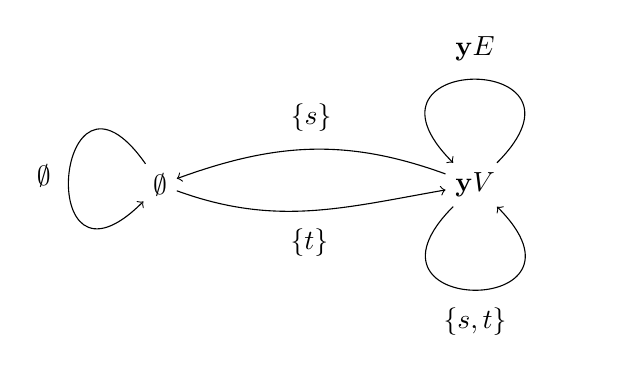
\begin{tikzpicture}
 \node (x) at (-2,0) {$\emptyset$};
 \node (y) at ( 2,0) {$\mathbf{y}V$};
 \path (x) edge [out=125, in=225, looseness=0.8, loop, distance=2cm, ->] node[left= 3pt] {$\emptyset$} (x);
 \path (y) edge [out= 45, in=135, looseness=0.8, loop, distance=2cm, ->] node[above=3pt] {$\mathbf{y}E$} (y);
 \path (y) edge [out=225, in=315, looseness=0.8, loop, distance=2cm, ->] node[below=3pt] {$\{s,t\}$} (y);
 \path (x) edge [out=340, in=190, ->] node[below=3pt] {$\{t\}$} (y);
 \path (y) edge [out=160, in=20, ->] node[above=3pt] {$\{s\}$} (x);
\end{tikzpicture}
\caption{The subobject classifier of $\mathscr{E}$}
\label{fig:subobject classifier for graph topos}
\end{figure}

The subobject classifier is thus given by
\[ \text{true} : 1 \to \Omega, \qquad v \mapsto \mathbf{y}V, \; e \mapsto \mathbf{y}E. \]
% If $X \in \mathscr{E}$ and $S \subseteq X$ a subgraph, then the classifying map $\chi_S : X \to \Omega$ works as follows:
% \begin{itemize}
% 	\item For each vertex $v \in X(V)$:
% 	\begin{itemize}
% 		\item If $v \not\in S(V)$, then $\chi_S(V)(v) = \emptyset$.
% 		\item If $v \in S(V)$, then $\chi_S(V)(v) = \mathbf{y}V$.
% 	\end{itemize}
% 	\item For each edge $e \in X(E)$:
% 	\begin{itemize}
% 		\item If $e \in S(E)$, then $\chi_S(E)(e) = \mathbf{y}E$.
% 		\item Else (we know that $e \not\in S(E)$):
% 		\begin{itemize}
% 			\item If $X(s)(e), X(t)(e) \in S(V)$, then $\chi_S(E)(e) = \{s,t\}$ (the edge is not in $S$, but both its source and target vertices are).
% 			\item Else if $X(s)(e) \in S(V)$, $X(t)(e) \not\in S(V)$, then $\chi_S(E)(e) = \{s\}$ (the edge is not in $S$, and only its source vertex is in $S$).
% 			\item Else if $X(s)(e) \not\in S(V)$ $X(t)(e) \in S(V)$, then $\chi_S(E)(e) = \{t\}$ (the edge is not in $S$, and only its target vertex is in $S$).
% 			\item Else $\chi_S(E)(e) = \emptyset$.
% 		\end{itemize}
% 	\end{itemize}
% \end{itemize}
% Basically, this works as you'd expect for subgraphs in a picture. You can leave out edges in a subgraph, but keep some of its target and source vertices.
% The negation operator $\neg : \Omega \to \Omega$ is a natural transformation with two components $\neg_V : \Omega V \to \Omega V$ and $\neg_E : \Omega E \to \Omega E$. They are defined as (cf. page 56 of Maclane\&Moerdijk)
% \[ \neg_V : \Omega V \to \Omega V, \qquad \neg_V(\emptyset) = \mathbf{y}V, \; \neg_V(\mathbf{y}V) = \emptyset, \]
% and
% \[ \neg_E : \Omega E \to \Omega E, \]
% explicitly calculated as
% \begin{align*}
% \neg_E(\emptyset) &= \mathbf{y}E, \\
% \neg_E(\mathbf{y}E) &= \emptyset, \\
% \neg_E(\{s\}) &= \emptyset\\
% \neg_E(\{t\}) &= \emptyset\\
% \neg_E(\{s,t\}) &= \emptyset\\
% \end{align*}
Now let $\mathscr{E}_{\lcf}$ be the Boolean topos of locally constant objects of $\mathscr{E}$. Since $\mathscr{E}_{\lcf}$ is Boolean, its subobject classifier is given by
\[ \Omega_{\lcf} = 1 + 1 \]
generated by the morphisms
\[ \text{true} : 1 \to \Omega, \qquad \text{false} = \neg \circ \text{true} : 1 \to \Omega. \]
So the graph $\Omega_{\lcf}$ looks like Figure \ref{fig:subobject classifier for lcf graph topos}.

\begin{figure}
\centering
\begin{tikzpicture}
 \node (x) at (-2,0) {$\emptyset$};
 \node (y) at ( 2,0) {$\mathbf{y}V$};
 \path (x) edge [out=125, in=225, looseness=0.8, loop, distance=2cm, ->] node[left= 3pt] {$\emptyset$} (x);
 \path (y) edge [out= 45, in=135, looseness=0.8, loop, distance=2cm, ->] node[above=3pt] {$\mathbf{y}E$} (y);
\end{tikzpicture}
\caption{The subobject classifier of $\mathscr{E}_{\lcf}$}
\label{fig:subobject classifier for lcf graph topos}
\end{figure}

Let $C_n$ be a cyclic graph with $n$ vertices and $n$ edges, $n > 0$. Then $C_n$ is locally constant finite; take $U$ to be the connected graph with $n$ vertices and $n-1$ edges. The product $C_n \times U$ is then a disjoint union of $n$ copies of $U$, so that we have an isomorphism $C_n \times U \cong \Delta(n) \times U$, where $\Delta(n)$ are $n$ copies of the graph with $1$ vertex and $1$ edge. Moreover, this isomorphism respects the projection down to $U$, so that $C_n$ is locally constant finite as per \cref{def:locally constant finite}.

I claim that disjoint unions of the $C_n$ are the only type of objects in $\mathscr{E}_{\lcf}$. Indeed, by \cref{prop:locally constant iff every restriction map is a bijection}, the restriction maps of an object $X \in \mathscr{E}_{\lcf}$ must be constant. This just translates to the fact that there are as many vertices as there are edges.

Moreover, each $C_n$ is an atom in $\mathscr{E}_{\lcf}$. Indeed, from the definition of $\Omega_{\lcf}$ we find that removing an edge means that we are forced to remove the vertices that the edge was attached to, too (this need not happen in $\mathscr{E}$). Thus $C_n$ has no subobjects other than the empty graph.

Next, we claim that every $C_n$ is also a Galois object. Indeed, there is a $\Z/n\Z$ action on the edges of $C_n$; simply cyclic shift the edges. Clearly then $\Aut(C_n) \cong C_n(E)$.
% Thus we may conclude that
% \begin{claim}
% Let $\mathbf{G}$ be the full subcategory of $\mathbf{I}$ whose objects are Galois. Then every object of $\mathbf{G}$ is of the form $(C_n,e)$ for some $n > 0$.
% \end{claim}
% \begin{proof}
% Write $C_n(V) = \{v_0,\ldots,v_{n-1}\}$ and $C_n(E) = \{e_0,\ldots,e_{n-1}\}$. Then $\Aut(C_n) = \Z/n\Z$, with action given by $m \cdot e_j = e_{j + m \bmod{n}}$. Hence $\Aut(C_n) \cong p^*(C_n)$, so $\mathbf{G}$ certainly contains all the $(C_n,e)$. Conversely suppose that $(A,e) \in \mathbf{G}$. Let $\varphi : A \times U \to \Delta n \times U$ be an isomorphism over $U$, where $U \to 1$ has global support. Note that $\# A = \# \Delta n = n$. Let $v \in A$ be a vertex. Let $\partial^+(v)$ be the number of incoming edges into the vertex $v$. Assume that $\partial^+(v) = 0$. Then for all $(v,u) \in A \times U$ we also have $\partial^+(v,u) = 0$. However $\varphi(v,u) = (v_j,u)$ for some $v_j \in C_n$, and $\partial^+(v_j,u) > 0$ for some $u \in U(V)$. This is in contradiction with $\partial^+(v,u) = 0$ for all $u \in U(V)$. So we conclude that $\partial^+(v) > 0$ for all $v \in A(V)$. This forces $\partial^+(v) = 1$ for all $v \in A(V)$, because $n = \sum_{v \in A(V)} \partial^+(v)$. Since we didn't use the fact that these edges are incoming, the same argument shows that the number of outgoing edges is also $1$ for each $v \in A(V)$. Finally, since $A$ is connected we may conclude that $A = C_n$.
% \end{proof}
% So the cycles form a cofinal subcategory of $\mathbf{I}$. 
Thus we may conclude that
\[ \pi_1(\mathscr{E}, E) = \lim_{\leftarrow n} \Aut(C_n) \cong \lim_{\leftarrow n} \Z/n\Z = \widehat{\Z}. \]
It is to be noted that if we chose a different point of $\mathscr{E}$, say the object $V$, using \cref{constr:how to get points}, we would end up with the same argumentation; there's a  $\Z/n\Z$ action on the vertices, and it can only be a $\Z/n\Z$ action because the source and target vertices of the edges of $C_n$ must match up.

% \section{Worked Example}

% Take a 

% An $n$-simplex $\sigma$ of a simplicial set $S$ is called \emph{degenerate} if there exists an $m < n$ and an order-preserving surjection $f : \mathbf{n} \to \mathbf{m}$ and an $m$-simplex $\tau$ of $S$ such that $\sigma = (Sf)(\tau)$. Note that $0$-simplices (vertices) are never degenerate. An $n$-simplex $\sigma$ is called \emph{non-degenerate} if it is not degenerate.

% \begin{lemma}[Eilenberg-Zilber]
% \label{lem:eilenberg-zilber} Let $S \in \mathbf{SSets}$. For each $n$-simplex $\sigma \in S_n$ there exists a unique order-preserving surjection $f : \mathbf{n} \to \mathbf{m}$ and a unique non-degenerate $m$-simplex $\tau \in S_m$ such that $\sigma = (Sf)(\tau)$.
% \end{lemma}
% \begin{proof}
% \begin{color}{red} Put a reference here... \end{color}
% If $\sigma$ is already non-degenerate, take $m=n$ and $f = \id$. If $\sigma$ is degenerate, then there exists some surjection $f_1 : [n] \to [m_1]$ with $m_1 < n$ and an $m_1$-simplex $\sigma_1$ such that $\sigma = (Sf_1)(\sigma_1)$. If $\sigma_1$ is non-degenerate, we are done. Otherwise, continue in this way until we reach a $\sigma_j$ that is non-degenerate. This process ends eventually since with each iteration, $m_i < m_{i-1}$, and vertices are always non-degenerate.
% So the existence of such a pair $(f,\tau)$ with $\sigma = (Sf)(\tau)$ is established. Suppose then that $(f',\tau')$ is another pair with $\sigma = (Sf')(\tau')$. Consider the pushout
% \[ \begin{tikzcd}
% \left[n\right] \arrow{r}{f} \arrow[swap]{d}{f'} & \left[m\right] \arrow{d}{\pi} \\
% \left[m'\right] \arrow[swap]{r}{\pi'} & \left[p\right]
% \end{tikzcd} \]
% in $\mathbf{\Delta}$. We can apply the Yoneda functor to get a commutative diagram
% \[ \begin{tikzcd}
% \mathbf{\Delta}\left(-,\left[n\right]\right) \arrow{r}{\mathbf{\Delta}\left(-,f\right)} \arrow[swap]{d}{\mathbf{\Delta}\left(-,f'\right)} & \mathbf{\Delta}\left(-,\left[m\right]\right) \arrow{d}{\mathbf{\Delta}\left(-,\pi\right)} \\
% \mathbf{\Delta}\left(-,\left[m'\right]\right) \arrow[swap]{r}{\mathbf{\Delta}\left(-,\pi'\right)} & \mathbf{\Delta}\left(-,\left[p\right]\right)
% \end{tikzcd} \]
% in $\mathbf{SSet}$. This diagram is still a pushout. While the $n$-simplex $\sigma$ is an element of the set $S_n$, it may equivalently be regarded as a functor $\sigma : \mathbf{\Delta}(-,[n]) \to S$ describing how the simplex is laid into the simplicial set. Similarly for $\tau$ and $\tau'$. Hence we have a commutative diagram
% \[ \begin{tikzcd}
% \mathbf{\Delta}\left(-,\left[n\right]\right) \arrow{r}{\mathbf{\Delta}\left(-,f\right)} \arrow[swap]{d}{\mathbf{\Delta}\left(-,f'\right)} & \mathbf{\Delta}\left(-,\left[m\right]\right) \arrow{d}{\mathbf{\Delta}\left(-,\pi\right)} \arrow[bend left]{ddr}{\tau} \\
% \mathbf{\Delta}\left(-,\left[m'\right]\right) \arrow[swap]{r}{\mathbf{\Delta}\left(-,\pi'\right)} \arrow[swap, bend right]{rrd}{\tau'} & \mathbf{\Delta}\left(-,\left[p\right]\right) \arrow[dotted]{dr}{\exists ! \rho} \\
% \; & \; & S
% \end{tikzcd} \]
% Since $\tau \circ \mathbf{\Delta}(-,f) = \sigma = \tau' \circ\mathbf{\Delta}(-,f')$, there exists a unique mediating $\rho$ such that $\mathbf{\Delta}(-,\pi) \circ \rho = \tau$ and $\mathbf{\Delta}(-,\pi') \circ \rho = \tau'$ as indicated by the dotted arrow. We can regard $\rho$ equivalently as a $p$-simplex in the set $S_p$, while $\pi$ and $\pi'$ are order-preserving surjections. So we see that $\tau = (S \pi)(\rho)$ and $\tau' = (S \pi')(\rho)$. But $\tau$ and $\tau'$ are both non-degenerate. So we must have $\pi = \pi' = \id$, $m=p=m'$, and hence $\tau = \tau'$.
% \end{proof}



